% © Copyright Brayden Price 2024

% This file is part of Brayden's AP Calculus AB Notes.

% Brayden's AP Calculus AB Notes is free software: you can redistribute it and/or modify it under the terms of the GNU General Public License as published by the Free Software Foundation, either version 3 of the License, or (at your option) any later version.

% Brayden's AP Calculus AB Notes is distributed in the hope that it will be useful, but WITHOUT ANY WARRANTY; without even the implied warranty of MERCHANTABILITY or FITNESS FOR A PARTICULAR PURPOSE. See the GNU General Public License for more details.

% You should have received a copy of the GNU General Public License along with Brayden's AP Calculus AB Notes. If not, see <https://www.gnu.org/licenses/>.

\documentclass[12pt,letterpaper, onecolumn]{exam}
\usepackage{amsmath}
\usepackage{amssymb}
\usepackage{nicefrac}
\usepackage{graphicx}
\usepackage{tocbasic}
\usepackage{hyperref}
\usepackage{signchart}
\usepackage{mathtools}

\usepackage{xcolor}
\hypersetup{
	colorlinks=true,
	linkcolor=blue,
	filecolor=magenta,      
	urlcolor=cyan,
}

\usepackage[lmargin=71pt, tmargin=1.2in]{geometry}  %For centering solution box
\lhead{AP Calculus AB -- APC 4.3 -- 4.4 Assignment\\}
\rhead{Brayden Price\\}
% \chead{\hline} % Un-comment to draw line below header
\thispagestyle{empty}   %For removing header/footer from page 1
\newcommand\at[2]{\left.#1\right|_{#2}}


\DeclareNewTOC[%
type=exercise,%
types=exercises,%
name=Exercise,%
listname={List of Questions},%
tocentrystyle=tocline,%
tocentryindent=0pt,%
tocentrydynnumwidth,%
tocentrypagenumberformat=\entryprefix{page~},%
tocentrypagenumberbox=\mbox
]{exr}
\newcommand*\entryprefix[2]{#1#2}

\newdimen\tcolw \tcolw=2.5em % the column width
\edef\ecatcode{\catcode`&=\the\catcode`&\relax}\catcode`&=4
\def\sgchart#1#2{\vbox{\offinterlineskip\halign{\hfil##\quad&##\hfil\crcr\sgchartA#2,:,%
			\omit\sgchartR&\kern.2pt\sgchartS{.5\tcolw}\relax\sgchartE#1,\relax,%
			\sgchartS{.5\tcolw}\relax\cr
			\noalign{\kern2pt}&\def~{}\kern.5\tcolw\sgchartD#1,\relax,\cr}}}
\def\sgchartA#1:#2,{\cr\ifx,#1,\else $#1$&\sgchartB#2{}\expandafter\sgchartA\fi}
\def\sgchartB#1{\hbox to\tcolw{\hss$#1$\hss}\sgchartC}
\def\sgchartC#1{\ifx,#1,\else
	\strut\vrule\kern-.4pt\hbox to\tcolw{\hss$#1$\hss}\expandafter\sgchartC\fi}
\def\sgchartD#1#2,{\ifx\relax#1\else\hbox to\tcolw{\hss$#1#2$\hss}\expandafter\sgchartD\fi}
\def\sgchartE#1#2,{\ifx\relax#1\else
	\ifx~#1\sgchartS\tcolw\circ \else\sgchartS\tcolw\bullet\fi \expandafter\sgchartE\fi}
\def\sgchartR{\leaders\vrule height2.8pt depth-2.4pt\hfil}
\def\sgchartS#1#2{\hbox to#1{\kern-.2pt\sgchartR \ifx\relax#2\else
		\kern-.7pt$#2$\kern-.7pt\sgchartR\fi\kern-.2pt}}
\ecatcode

\qformat{%
	\textbf{Question~\thequestion}%
	\addxcontentsline{exr}{exercise}{Question~\thequestion}%
	\hfill\thepoints%
}

% Command for Line Segment 
\newcommand{\lineSeg}[1]{\overline{\mathrm{#1}}}

\begin{document}
	
	\begingroup  
	\centering
	\LARGE AP Calculus AB\\
	\LARGE AP Classroom: 5.1 -- 5.3\\[0.5em]
	\large \today\\[0.5em]
	\large Brayden Price \\
	All final solutions are \boxed{boxed} \\
	Only FRQs are included (for now). \\
	\endgroup
	\rule{\textwidth}{0.4pt}
	
	\listofexercises
	\clearpage
	
	\printanswers
	\renewcommand{\solutiontitle}{\noindent\textbf{Solution:}\enspace}   %Replace "Ans:" with starting keyword in solution box
	
	\begin{questions}
		
		\question 
		$$f(t) = \begin{cases}
			 48t + t^2 - \frac{t^3}{12}, & \text{for } 0 \leq t < 6 \\
			 g(t)						 & \text{for } 6 \leq t \leq 12
		\end{cases}$$
		\begin{center}\begin{tabular}{|l||l|l|l|l|}
			\hline
			$t$ (hours)           & 6   & 8   & 10  & 12  \\ \hline
			$g(t)$ (cubic meters) & 306 & 376 & 428 & 474 \\ \hline
		\end{tabular}\end{center}
		At an excavation site, the amount of dirt that has been removed, in cubic meters, is modeled by the function $f$ defined above, where $g$ is a differentiable function and $t$ is measured in hours. Values of $g(t)$ at selected values of $t$ are given in the table above.
		\begin{parts}
			\part According to the model $f$, what is the average rate of change of the amount of dirt removed over the time interval  $6 \leq t \leq 12$ hours?
			\part Use the data in the table to approximate $f^{\prime}(9)$, the instantaneous rate of change in the amount of dirt removed, in cubic meters per hour, at time $t=9$ hours. Show the computations that lead to your answer.
			\part Is $f$ continuous for $0 \leq t \leq 12$? Justify your answer.
			\part   Find $f^{\prime}(t)$, the instantaneous rate of change in the amount of dirt removed, in cubic meters per hour, at time $t=2$ hours.
		\end{parts}
		
		\begin{solution}
			\begin{parts}
				\part Since $f(t)$ is defined by the $g(t)$ over $0 \leq t < 6$, we can use values in the table of $g$ to find the AROC.
				$$\text{AROC} = \frac{g(12)-g(6)}{12-6} = \boxed{\frac{474-306}{6} \text{ m\textsuperscript{3} / min}}$$ 
				(answer could be simplified but is not necessary to earn point)
				
				\part $f^\prime(9)$ can be approximated using AROC over a neighboring interval, like $8 \leq t \leq 10$. \\
				Since $f(t)$ is defined by $g(t)$ for $6 \leq t \leq 12$, we should use that to find our AROC.
				$$\text{AROC} = \frac{g(10)-g(8)}{10-8} = \boxed{\frac{428-376}{2} \text{ m\textsuperscript{3} / min} \approx f^\prime(9)}$$ (see above note about simplification)
				
				\part Since $g$ is differentiable and $f(t)$ is defined by a polynomial over $0 \leq t < 6$, both individual intervals are continuous. We must check the continuity at $t=6$, however.
				$$\lim_{t \to 6^-} = 48(6) + 6^2 - \frac{6^3}{12} = 288 + 36 - 18 = 306$$
				$$\lim_{t \to 6^+} = g(6) = 306$$
				$$\therefore \lim_{t \to 6^-} = \lim_{t \to 6^+} = g(6)$$ 
				$\therefore \boxed{f(t)\text{ is continuous for } 0 \leq t \leq 12 }$ since it is continuous at $t=6$ and on $0 \leq t < 6$ and $6 < t \leq 12$.
				
				\part $$f^\prime(t) = 48 + 2t - \frac{t^2}{4} \text{ for } 0 \leq t \leq 6$$
				$$f^\prime(2) = 48 + 4 - \frac{4}{4} = \boxed{51}$$
			\end{parts}
		\end{solution}
		
		\setcounter{question}{6} \question Just a note: this question is here in error because it uses integrals, which we haven't learned yet.
		
		\setcounter{question}{9} \question Let f be the function given by the $f(x) = \frac{\ln x}{x}$ for all x > 0. The derivative of f is given by $f^\prime(x) = \frac{1-\ln x}{x^2}$. \\
		Find the $x$-coordinate of the critical point of $f$. Determine whether this point is a relative minimum, a relative maximum, or neither for the function $f$. Justify your answer.
		\begin{solution}
			$f^\prime(x)$ must be undefined or zero to constitute a critical point. 
			The only undefined point, $x=0$, is excluded (not in the domain of $f(x)$).
			So, set numerator equal to zero and solve:
			$$1-\ln x = 0 \Rightarrow \ln x = 1 \Rightarrow \log_e x = 1 \Rightarrow e^1 = x$$
			At point $x=e$, $f^\prime(x) = 0$ and $f(x)$ is defined, so $\boxed{x=e \text{ is a critical point.}}$
			
			\begin{gather*}
				\frac{1-\ln(e^2)}{(e^2)^2} =\frac{1-2}{e^4} = - \frac{1}{e^4} \\
				\frac{1-\ln(e^0)}{(e^0)^2} = 1-0 = 1 \\ \\
				\sgchart {e} {f'(x): +-}
			\end{gather*}
			\begin{multline*}
				f^\prime(x) > 0 \text{ when } 0 < x < e \text{ and } f^\prime(x) < 0 \text{ when } x > e. \\
				\text{ Therefore, } \boxed{x = e \text{ must be a maximum on } f}.
			\end{multline*}
		\end{solution}
		
		\setcounter{question}{11} \question Let $f$ be defined by $f(x)=3x^5-5x^3+2$.
		\begin{parts}
			\part On what intervals is $f$ increasing?
			\part On what intervals is the graph of $f$ concave upward?
			\part Write the equation of each horizontal tangent line to the graph of $f$.
		\end{parts}
		
		\begin{solution}
			\begin{parts}
				\part 
				\begin{gather}
				\begin{align} 
					f^\prime(x) &= 15x^4 - 15x^2 \\
								&= 15x^2(x^2-1) \\
					x			&= \left\lbrace 0 , \pm 1 \right\rbrace
				\end{align}\\
					\sgchart {-1,0,+1} {f^\prime(x): +--+}
				\end{gather}
				$f^\prime(x) > 0 \  \boxed{\text{on } (-\infty,0) \text{ and } (1,+\infty)}$, therefore, f is increasing \\
				on these intervals.
				
				\part 
				\begin{gather}
					\begin{align} 
						f^{\prime\prime}(x) &= 60x^3 - 30x \\
						&= 30x(2x^2-1) \\
						x			&= \left\lbrace 0 , \pm \frac{\sqrt{2}}{2} \right\rbrace
					\end{align}\\
					\sgchart {-\frac{\sqrt{2}}{2}, 0, +\frac{\sqrt{2}}{2}} {f^{\prime\prime}(x): -+-+}
				\end{gather}
				$f^{\prime\prime}(x) > 0 \  \boxed{\text{on } (-\frac{\sqrt{2}}{2},0) \text{ and } (+\frac{\sqrt{2}}{2},+\infty)}$, therefore, f is increasing \\
				on these intervals
				
				\part \hfill
				Horizontal tangent lines have a slope of zero. 
				Set $f^\prime(x)$ to zero and solve:
				\begin{gather}
					f^\prime(x) = 15x^4 - 15x^2 \\
					15x^4 - 15x^2 = 0 \\
					15x^2(x^2 - 1) = 0 \\ 
					x = \left\lbrace \pm 1 , 0 \right\rbrace
				\end{gather}
					Those are the x-coordinates of the points of tangency where the slope is zero. \\
					Now we have to find the y-coordinates of those points (since horizontal lines have form $y=\text{some number}$
				\begin{align}
					f(-1) &= 3(-1)^5 - 5(-1)^3 + 2 = -3 + 5 + 2 = 4 \\
					f(0) &= 2 \\
					f(1) &= 3(1)^5 - 5(1)^5 + 2 = 3 - 5 + 2 = 0 
				\end{align}
				Points of tangency: $(-1,4), (0,2), (1,0)$ \\
				$\boxed{y=4, y=0, \text{and } y=2}$ are the horizontal tangent lines to the graph $f$.
			\end{parts}
		\end{solution}
		
		\setcounter{question}{14} \question Let f be a function that is \underline{even} and continuous on the closed interval $[−3,3]$. The function $f$ and its derivatives have the properties indicated in the table below.
		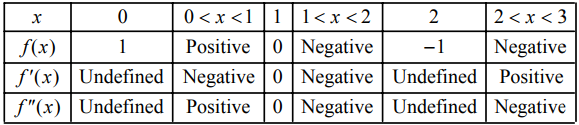
\includegraphics[width=0.6\linewidth]{question15_001}
		
		\begin{solution}
			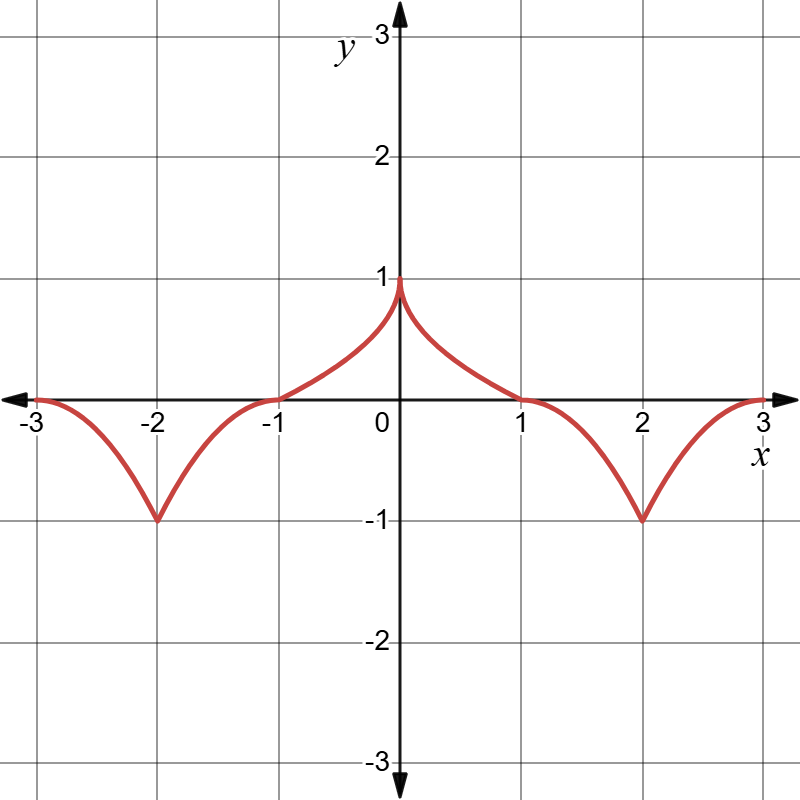
\includegraphics[width=0.6\linewidth]{question15_002}
		\end{solution}
		
		\setcounter{question}{19} \question Consider the curve given by $x^2-xy+2y^2=7$.
		\begin{parts}
			\part Show that $\frac{dy}{dx} = \frac{y-2x}{4y-x}$
			\part Determine the $y$-coordinate of each point on the curve at which the line tangent to the curve at that point is vertical. Justify your answer.
			\part Find $\frac{d^2y}{dx^2}$ in terms of $x$, $y$, and $\frac{dy}{dx}$. The line tangent to the curve at the point $(1,2)$ is horizontal. Determine whether the curve is concave up or concave down at the point $(1,2)$.
		\end{parts}
		
		\begin{solution}
			\begin{parts}
				\part 
				\begin{gather*}
					\frac{d}{dx} \left( x^2-xy+2y^2 \right) = \frac{d}{dx} ( 7 ) \\
					2x - (y + x{y^\prime}) + 4y{y^\prime} = 0 \\
					2x - y - x{y^\prime} + 4y{y^\prime} \\
					2x - y = {y^\prime} ( x - 4y ) \\
					{y^\prime} = \frac{2x - y}{x - 4y} = \frac{y - 2x}{4y - x}
				\end{gather*}
				\part Vertical tangent lines have undefined slope, meaning the denominator of the derivative of the curve must equal zero. \\
				$4y-x=0$ \ $\Rightarrow$ \  $x=4y$ \\
				Plug into curve:
				\begin{align*}
					7 &= (4y)^2 - (4y)y +2y^2 \\
					7 &= 16y^2 - 4y^2 + 2y^2 \\
					7 &= 14y^2 \\
					y^2 &= \frac{1}{2} \\
					y &= \pm \sqrt{\frac{1}{2}}
				\end{align*}
				
				\part 
				\begin{multline*}
					\frac{d^2y}{dx^2} = \frac{d}{dx} \left( \frac{dy}{dx} \right)  = \frac{d}{dx} \left( \frac{y - 2x}{4y - x} \right) \\
					 = \frac{ \left( y-2x \right)^\prime \left( 4y-x \right) - \left( 4y - x \right)^\prime \left( y - 2x \right)}{ \left( 4y - x  \right)^2 } \\
					 = \boxed{\frac{ (y^\prime - 2)(4y-x) - (4y^\prime - 1)(y-2x) } { (4y-x)^2 }}
				\end{multline*}
				Find $y^\prime$ at $(1,2)$:
				$$y^\prime \ \bigg{|}_{(1,2)} = \frac{2 - 2(1)}{4(2) - 1} = \frac{0}{7} = 0$$
				Plug in $y^\prime$ and $(1,2)$ to $y^{\prime\prime}$:
				\begin{align*}
					y^{\prime\prime} \ \bigg{|}_{(1,2)} &= \frac{ (0 - 2)(4(2)-1) - (4(0) - 1)((2)-2(1)) } { (4(2)-1)^2 }
									 &= \frac{ (-2)(7) - (-1)(0) } { (7)^2 }
									 &= \boxed{-\frac{ 14 } { 49 }}
				\end{align*}
				Therefore, $y^\prime$ is \boxed{\text{concave down}} at $(1,2)$ because $y^{\prime\prime}<0$
			\end{parts}
		\end{solution}
		
	\end{questions}
\end{document}